\documentclass{article}
\usepackage[utf8]{inputenc}
\usepackage[spanish]{babel}
\usepackage{listings}
\usepackage{graphicx}
\graphicspath{ {images/} }
\usepackage{cite}

\begin{document}

\begin{titlepage}
    \begin{center}
        \vspace*{1cm}
            
        \Huge
        \textbf{Parcial N° 1}
            
        \vspace{2 cm}
        \LARGE
    
            
        \vspace{2 cm}
            
        \textbf{Ivonne  Rosero }\\
        \large
        1007687589
        
        \vspace{2cm}
        \LARGE
        
        \textbf{Rigoberto Berrio}\\
        \large
        1040327583
            
        \vfill
            
        \vspace{0.8cm}
            
        \Large
        Despartamento de Ingeniería Electrónica y Telecomunicaciones\\
        Universidad de Antioquia\\
        Medellín\\
        Abril de 2021
            
    \end{center}
\end{titlepage}

\tableofcontents
\newpage
\section{Análisis del problema y consideraciones para la alternativa de solución propuesta.}\label{intro}
 
Gracias a los apuntes y grabaciones de clase se estan haciendo pruebas para afianzar el conocimiento para poder asimilarlo  al nivel del examen.

Decidimos utilizar 8 integrados para que cada uno controlara 8 leds y asi completar los 64 leds requeridos.

En la Figura (\ref{fig:circuito}) se muestra el circuito a utilizar en el examen.
\begin{figure}[h]
\includegraphics[width=12cm]{circuito.jpg}
\centering
\caption{Circuito final}
\label{fig:circuito}
\end{figure}


\section{Esquema que describa las tareas que se definieron en el desarrollo del algoritmo.}\label{intro}



\section{Esquema donde describa las tareas que se definieron en el desarrollo del algoritmo.}\label{intro}

\newpage
\section{Algoritmo implementado.}\label{intro}
Algoritmo base.
\begin{figure}[h]
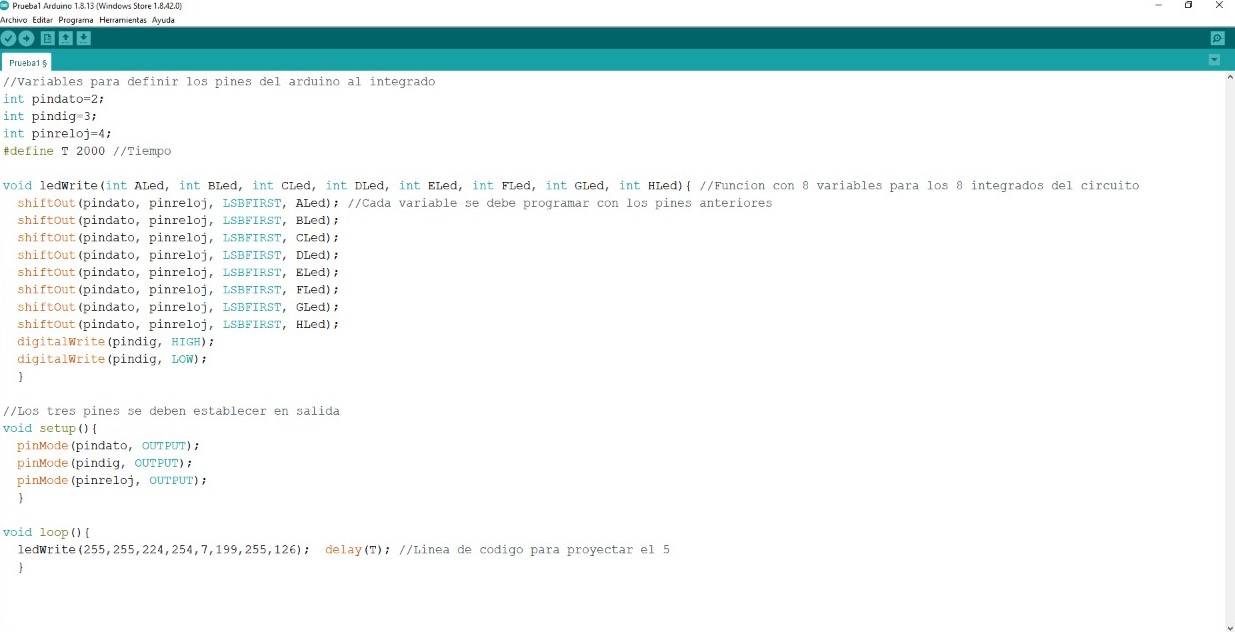
\includegraphics[width=12cm]{Algoritmo.jpeg}
\centering
\caption{Algoritmo Implementado}
\label{fig:Algoritmo}
\end{figure}

\newpage
\section{Problemas de desarrollo.}\label{intro}
Se usa el comando shiftOut() la cual se encarga de desplazar hacia la salida un bit cada vez, comienza a partir del bit mas significativo o menos significativo en este caso se inicio desde el bit  menos significativo usando el comando LSBFIRST.

Se programaron los 3 pines que van conectados del arduino al integrado en OUTPUT (salida).

Se obtiene que los leds formen la figura.

\begin{figure}[h]
\includegraphics[width=10cm]{figura #5.jpeg}
\centering
\caption{Figura final}
\label{fig:figura #5}
\end{figure}

Siempre que el usuario ingrese alguna opcion siempre aparecera de la primero la figura.

\newpage
\section{Evolución del algoritmo y consideraciones a tener en cuenta en la implementación.}\label{intro}
Se crea un menu de manera que el usuario se le facilite la opcion que quiera elegir.

\begin{figure}[h]
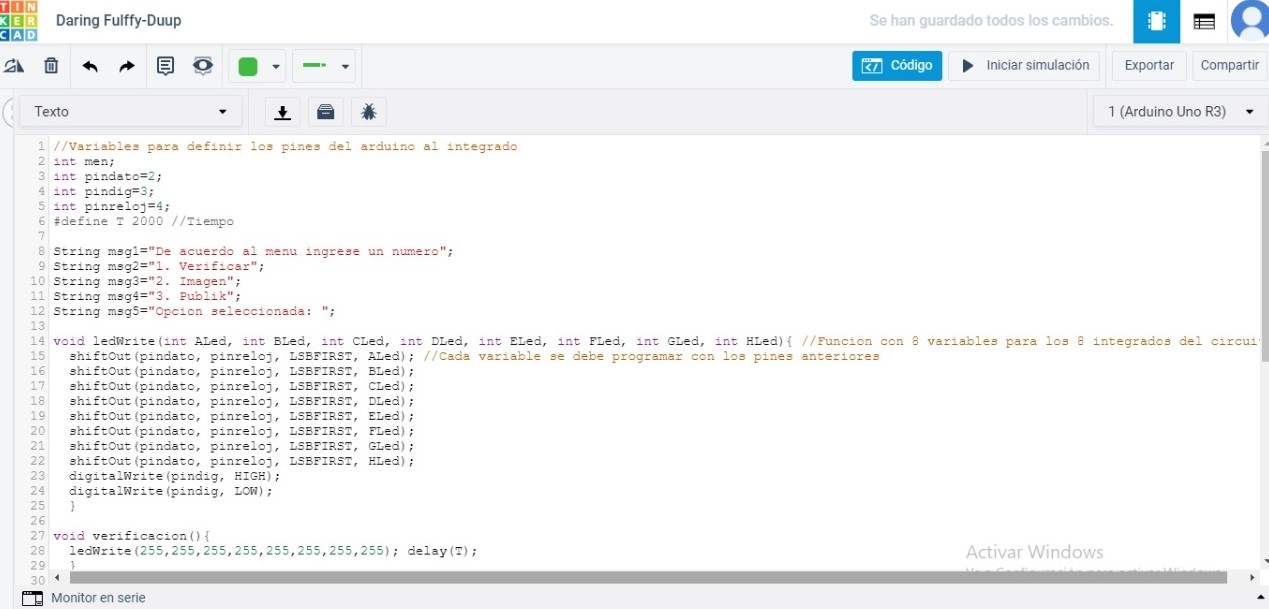
\includegraphics[width=10cm]{Avance 1.jpeg}
\centering
\caption{Avance del codigo}
\label{fig:Avance 1}
\end{figure}








\end{document}
